\documentclass{article}
\usepackage[utf8]{inputenc}

\usepackage{tikz}
\usetikzlibrary{automata, positioning, arrows}

\begin{document}

\begin{figure}[h!]
	\centering
	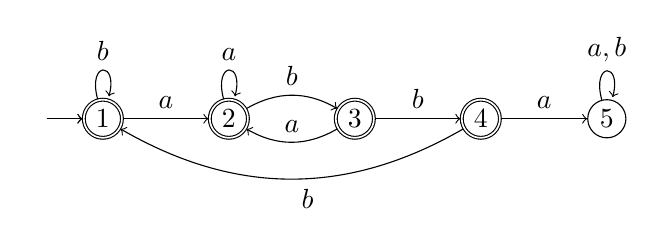
\begin{tikzpicture}[node distance=16mm, every state/.style={minimum size=4mm, inner sep=2pt}]
		\node[state,initial,initial,initial text={},accepting] (1) {$1$};
		\node[state,accepting] (2)  [right of=1]  {$2$};
		\node[state,accepting] (3) [right of=2] {$3$};
		\node[state,accepting] (4)  [right of=3]  {$4$};
		\node[state] (5)  [right of=4]  {$5$};
		
		\path[->] 
		(1) edge [loop above] node {$b$} ()
		(1) edge node [above] {$a$} (2)
		(2) edge [loop above] node {$a$} ()
		(2) edge [bend left] node [above] {$b$} (3)
		(3) edge [bend left] node [above] {$a$} (2)
		(3) edge node [above] {$b$} (4)
		(4) edge [bend left] node [below right] {$b$} (1)
		(4) edge node [above] {$a$} (5)
		(5) edge [loop above] node [above] {$a,b$} ();
	\end{tikzpicture}
\caption{solution}
\label{fig:nfa_no_abba}
\end{figure}

\begin{figure}[h!]
	\centering
	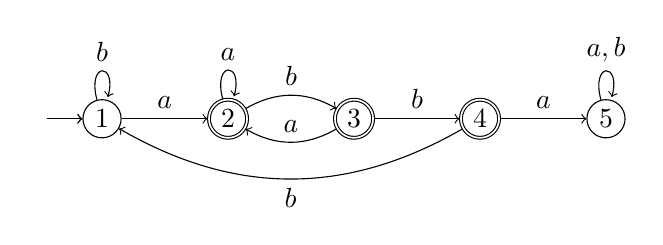
\begin{tikzpicture}[node distance=16mm, every state/.style={minimum size=4mm, inner sep=2pt}]
		\node[state,initial,initial,initial text={}] (1) {$1$};
		\node[state,accepting] (2)  [right of=1]  {$2$};
		\node[state,accepting] (3) [right of=2] {$3$};
		\node[state,accepting] (4)  [right of=3]  {$4$};
		\node[state] (5)  [right of=4]  {$5$};
		
		\path[->] 
		(1) edge [loop above] node {$b$} ()
		(1) edge node [above] {$a$} (2)
		(2) edge [loop above] node {$a$} ()
		(2) edge [bend left] node [above] {$b$} (3)
		(3) edge [bend left] node [above] {$a$} (2)
		(3) edge node [above] {$b$} (4)
		(4) edge [bend left] node [below] {$b$} (1)
		(4) edge node [above] {$a$} (5)
		(5) edge [loop above] node [above] {$a,b$} ();
	\end{tikzpicture}
\caption{automaton1}
\label{fig:error_3}
\end{figure}

\begin{figure}[h!]
	\centering
	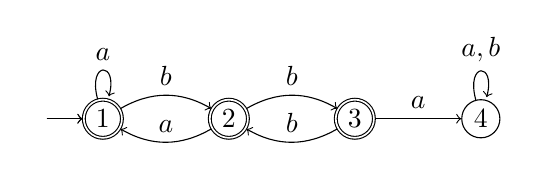
\begin{tikzpicture}[node distance=16mm, every state/.style={minimum size=4mm, inner sep=2pt}]
		\node[state,initial,initial,initial text={},accepting] (1) {$1$};
		\node[state, accepting] (2)  [right of=1]  {$2$};
		\node[state, accepting] (3) [right of=2] {$3$};
		\node[state] (4)  [right of=3]  {$4$};
		
		\path[->] 
		(1) edge [loop above] node {$a$} ()
		(1) edge [bend left] node [above] {$b$} (2)
		(2) edge [bend left] node [above] {$a$} (1)
		(3) edge [bend left] node [above] {$b$} (2)
		(2) edge [bend left] node [above] {$b$} (3)
		(3) edge node [above] {$a$} (4)
		(4) edge [loop above] node [above] {$a,b$} ();
	\end{tikzpicture}
\caption{automaton2}
\label{fig:error_5}
\end{figure}

\end{document}
